\documentclass[conference]{IEEEtran}
% \IEEEoverridecommandlockouts
% The preceding line is only needed to identify funding in the first footnote. If that is unneeded, please comment it out.
%Template version as of 6/27/2024

\usepackage{cite}
\bibliographystyle{IEEEtran}
\usepackage{amsmath,amssymb,amsfonts}
\usepackage{algorithmic}
\usepackage{graphicx}
\usepackage{textcomp}
\usepackage{xcolor}

\newcommand{\T}{^\top}
\newcommand{\tr}{\textrm{tr}}
\renewcommand{\vec}[1]{\boldsymbol{\mathbf{#1}}}
\newcommand{\defeq}{\triangleq}

\def\BibTeX{{\rm B\kern-.05em{\sc i\kern-.025em b}\kern-.08em
    T\kern-.1667em\lower.7ex\hbox{E}\kern-.125emX}}
\begin{document}

\title{Fault-Tolerant Attitude Control of a Cubesat\\
{\footnotesize \textsuperscript{*}Note: Sub-titles are not captured for https://ieeexplore.ieee.org  and
should not be used}
\thanks{Identify applicable funding agency here. If none, delete this.}
}

\author{\IEEEauthorblockN{1\textsuperscript{st} Given Name Surname}
\IEEEauthorblockA{\textit{dept. name of organization (of Aff.)} \\
\textit{name of organization (of Aff.)}\\
City, Country \\
email address or ORCID}
\and
\IEEEauthorblockN{2\textsuperscript{nd} Given Name Surname}
\IEEEauthorblockA{\textit{dept. name of organization (of Aff.)} \\
\textit{name of organization (of Aff.)}\\
City, Country \\
email address or ORCID}
}

\maketitle

\begin{abstract}

\end{abstract}

\begin{IEEEkeywords}
component, formatting, style, styling, insert.
\end{IEEEkeywords}

\section{Introduction}

Space is a growing industry with thousands in orbit currently and, with the introduction of satellite constellations, thousands more to come in the next decades. In this context automation of is key importance to keeping costs down. The attitude determination and control system (ACDS) enables a satellite to orient itself and is thus critical for operations such as communication and observation. Due to the inaccessible nature of orbit, ADCS fault-tolerant control (FTC) is an attractive method of allowing operations to continue after degradation or even failure of an actuator. Current industry standard methods of dealing with this problem involve putting the satellite into safe mode and solving the problem on the ground. This paper proposes to solve this problem online during operation using a fault detection and isolation unit (FDI) and an FTC unit.

\section{Problem Definition}

\section{Literature Review}

Here lies the literature review. Those who wander further beware.

\subsection{Satellite Attitude Kinematics}

\subsubsection{Attitude representations}
The satellite's orientation can be represented intuitively using euler angles such as yaw $\psi$, pitch $\theta$ and roll$\phi$. However these representations are not so effective for computation in attitude control as they require more expensive trigonometric functions to be used and produce singularities. The most accurate way to represent the attitude of an object is using the direction cosine matrix (DCM) aka. the rotation matrix. This is a 3x3 matrix where each column represents the orthogonal xyz axes vector. However this is cumbersome for computing calculations as it would require computing 9 differential equations to determine a satellite's attitude. Instead quaternions are used during computations. The quaternion can be defined as: 

\begin{equation}
    \begin{bmatrix}
        q_{1} \\ q_{2} \\ q_{3} \\ q_{4}
    \end{bmatrix}
    =
    \begin{bmatrix}
        e_{1}\sin(\Phi) \\ e_{2}\sin(\Phi) \\ e_{3}\sin(\Phi) \\ q_{4}\cos(\Phi)
    \end{bmatrix}
\end{equation}



\subsection{Attitude Control of a Satellite}
\subsubsection{Dynamics and Kinematics}
The attitude of a vehicle refers to it's orientation and angular rate in 3D space. In order to control a satellite's oritentation for pointing and other applications it's dynamics and kinemeatics must be understood and modelled. The motion of a satellite can be described by the kinematic equation \cite{sidiAttitudeDynamicsKinematics1997}:
\begin{equation}
    \vec{\dot{Q}}
=\frac{1}{2}
\begin{bmatrix}
q_{0} \ \ \neg q_{3} \ \ \ q_{2} \\ 
q_{3} \ \ q_{0} \ \ \ \neg q_{1} \\ 
\neg q_{2} \ \ q_{1} \ \ \ q_{0} \\ 
\neg q_{1} \ \ \neg q_{2} \ \ \ \neg q_{3} \\
\end{bmatrix} \vec{\omega_{b}}
\end{equation}

where $\vec{\omega_{b}}$ is the satellite's angular rate vector and $\vec{Q}$ is the quaternion representation of the satellite's attitude. 

A satellite's attitude with mass moment of inertia $\boldsymbol{J}$ can be modelled using the Newton-Euler equation \cite{sidiAttitudeDynamicsKinematics1997}: 

\begin{equation}
\mathbf{J}\mathbf{\dot{\vec{\omega_{b}}}} = \sum{\mathbf{T_{ext}}} -\mathbf{\vec{\omega_{b}}}\times(\mathbf{J}\vec{\omega_{b}}-\vec{h})-\vec{\dot{h}}
\end{equation}

where $\boldsymbol{\vec{\omega_{b}}}$ is the satellite's angular rate vector, $\boldsymbol{T_{ext}}$ is any external torque applied

\subsection{Quaternion Feedback Control}
A common control law designed used for 3-axis pointing control is the quaternion feedback control law. It uses proportional and derivative control to output a control signal $\vec{u}$ and is given by \cite{wieSpaceVehicleDynamics1998}:

\begin{equation}
    \vec{u} = -\vec{K_{q}}\vec{q_{e}} - \vec{K_{\omega}}\vec{\omega_{e}}
\end{equation}

where $\vec{K_{q}}$ and $\vec{K_{\omega_{b}}}$ are the quaternion and angular rate feedback gains respectively and $\vec{q_{e}}$ and $\vec{\omega_{e}}$ 
are the quaternion and angular rate errors respectively.

\subsection{Fault Detection and Isolation}
Fault detection and isolation (FDI) is crucial for providing up to date fault information for controller reconfiguration. In literature FDI is commonly used however in the case of Fault Tolerant Control diagnosis is an important step \cite{yinReviewRecentDevelopment2016}. Thus Fault Detection and Diagnosis (FDD) is a better metric and will be used in this work. An FDD high level algorithm can thus be summarized as asking the following questions:
\begin{itemize}
    \item Detection - has a fault occured?
    \item Isolation - what is the type and location of the fault?
    \item Diagnosis/Estimation - what is the value or magnitude of the fault?
\end{itemize}

Approaches to FDD can be broken down into 2 broad categories: model-based and data-driven. Some common methods of FDI include:
\begin{itemize}
    \item Decision trees
    \item Bayesian networks
    \item Neural networks
\end{itemize}

\subsection{Fault Tolerant Control}
Existing design techniques for FTC can be classified into two approaches: passive FTC and active FTC. A passive FTC controller is designed to tolerate only a predefined, limited number of faults and does not require any online fault information. Passive FTC also does not require controller reconfiguration. \cite{yinReviewRecentDevelopment2016}

Active FTC, on the other hand, is designed to reconfigure the controller in the presence of a fault. It can achieve this through preselecting an existing control law or synthesizing a new control law. It therefore requires online fault detection and isolation (FDI) information. Degraded performance of the system does have to be accepted but the aim is to reduce conservativeness of the controller. \cite{yinReviewRecentDevelopment2016}
\subsubsection{Existing Problems in FTC}
\sethlcolor{green}
\hl{In \mbox{\cite{yinReviewRecentDevelopment2016}} the following open problems in FTC were identified}
\begin{itemize}
\item Existing attitude FTC is developed without considering spacecraft actuator nonlinearities
\item Existing attitude FTC has great conservativeness
\item Implementation of the existing attitude FTC requires angular velocity measurements
\item Existing FTC is without attitude fast slewing capability
\end{itemize}

\subsection{FTC Applied to Spacecraft}
In \cite{jiangAdaptiveBacksteppingFaulttolerant2010} a backstepping sliding-mode adaptive controller is designed to handle reaction wheel faults where a redundant actuator is available. unknown faults of the reaction wheels, external disturbances, and unknown inertia matrix of the spacecraft. 

Shen and collaborators \cite{shenActiveFaulttolerantControl2019} use backstepping to design a fault-tolerant controller for a satellite with reaction wheel faults taking into account saturation. The methodolgy in the later section of this paper of fault tolerant control in this paper closely follows this work.

\subsection{Backstepping}
To understand the work of Shen et al. \cite{shenActiveFaulttolerantControl2019} it is important to understand backstepping. In Non-linear Systems by H. Khalil \cite{khalilNonlinearSystems2002} backstepping is described as "a recursive design method for non-linear systems". It entails designing a series of virtual control inputs each of which stabilizes a subsystem and ultimately the overall system. The method is recursive in that the controller for the $i^{th}$ subsystem depends on the controller for the $(i-1)^{th}$ subsystem. It uses Lyapunov functions to stabilize each subsystem and generate a control law.

A high level overview of the technique can be described using a series of flow diagrams:



\subsubsection{Lyapunov Functions}
*A Lyapunov function is a scalar function that is positive definite and radially unbounded. It is used to prove the stability of a system. A Lyapunov function $V(x)$ is positive definite if $V(0)=0$ and $V(x)>0$ for all $x\neq0$. It is radially unbounded if $V(x)\rightarrow\infty$ as $x\rightarrow\infty$. A Lyapunov function is used to prove the stability of a system by showing that the time derivative of the Lyapunov function is negative definite. That is $\dot{V}(x)<0$ for all $x\neq0$. If this is true then the system is stable.

\par
Backstepping can be visualized with the following diagrams:

% \begin{figure}
%     \centering
%     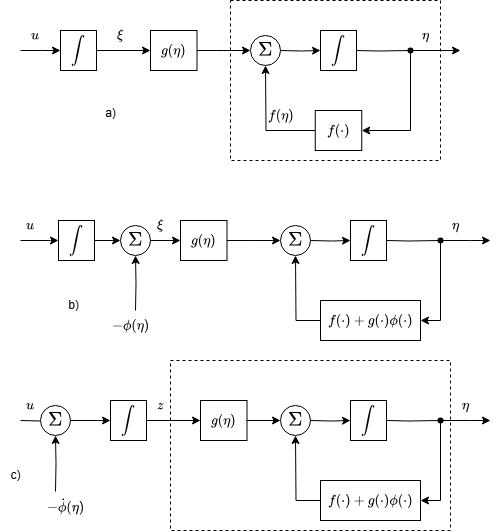
\includegraphics[width=0.5\textwidth]{Backstepping_diagram.drawio.png}
%     \caption{Backstepping Diagram}
%     \label{fig:backstepping}
% \end{figure}

\subsection{Fault Tolerant Control Applied}

\section{Proposed Methodology}
\subsection{Fault Detection and Diagnosis}
For the purposes of this paper, the FDI unit will not be implemented. Instead, the fault will be injected directly into the system and the FTC unit will be used to reconfigure the controller. Mathematically the estimated fault can be incorporated into the control law as follows:
\begin{equation}\vec{u}=(\mathbf{I}_{n}-\mathbf{E})\vec{u}_{c}+\vec{u}_{a}\end{equation}

where $E$ represents the effecitve loss of actuators $E=diag(e_{1},e_{2}\dots,e_{n})$ and $0\leq e_{i}\leq 1$. $e_{i}=0$ means the actuator is healthy. Additionally $\vec{u}_{a}$ represents the additive bias fault.

\subsection{Fault Tolerant Control}
The kinematic equation can be re-written in the following form \cite{shenActiveFaulttolerantControl2019}:

$\mathbf{S}(\vec{q})$ is the skew symmetric matrix, $\vec{q}=\begin{bmatrix}q_{1} \ q_{2} \ q_{3} \end{bmatrix}$ is the vector representation
\begin{equation}\mathbf{J}\dot{\vec{\omega}_{b}}=-\mathbf{S}(\vec{\omega}_{b})\mathbf{J}\vec{\omega}_{b}+\mathbf{D}\vec{u}+\vec{d}\end{equation}

\begin{equation} \dot{\mathbf{Q}}=\frac{1}{2}\begin{bmatrix}
\mathbf{S}(\vec{q})+q_{0}\mathbf{I}_{3} \\
-\vec{q}^{T}
\end{bmatrix} \vec{\omega}_{b}\end{equation}
$\vec{d}$ is the environmental disturbances
$\vec{\omega}_{b}$ is the body angular velocity in body fixed frame
$\mathbf{D}$ is actuator configuration matrix
$\mathbf{S(x)}$ represents the skew symmetric matrix 

\begin{equation}\vec{u}=(\mathbf{I}-\mathbf{E})\vec{u}_{c}+\vec{u}_{a}\end{equation}
where $E$ represents the effecitve loss of actuators $E=diag(e_{1},e_{2}\dots,e_{n})$ and $0\leq e_{i}\leq 1$. $e_{i}=0$ means the actuator is healthy. $\vec{u}_{a}$ additive bias fault.


\begin{equation}
    \mathbf{J}\dot{\vec{\omega}_{b}}=-\mathbf{S}(\vec{\omega}_{b})\mathbf{J}\vec{\omega}_{b}+\mathbf{D}\vec{u}_{c}+\vec{f}+\vec{d}
\end{equation} 
where $\vec{f}=\mathbf{D}\mathbf{E}\vec{u}_{c}+\mathbf{D}\vec{u}_{a}$ represents the influence of the fault on the system and acts as a disturbance on the system.


let $\Delta \vec{f}=\vec{f}-\vec{\hat{f}}$ be the estimation error and $\Delta \vec{f}$ is bounded



$\mathbf{D}^+=\mathbf{D}^T(\mathbf{D}\mathbf{D}^T)^{-1}$ is the pseudo inverse matrix

In \cite{shenActiveFaulttolerantControl2019} a non-linear virtual control input is chosen based on the paper by \cite{kimRobustBacksteppingControl2003}. This improves the torque profile and motion around the equilibrium point. The virtual control input is given by:

\begin{equation}\vec{\omega}_{c}=-\alpha\arctan(\beta\vec{q})\end{equation}

\begin{equation}\vec{s}=\vec{\omega_{b}}-\vec{\omega_{c}}=\vec{\omega_{b}}+\alpha\arctan(\beta\vec{q})\end{equation}

A Lyapunov function is chosen as 

\begin{equation}V_{1}=k_{0}\vec{q}^T\vec{q}+k_{0}(1-q_{0})^T\end{equation}

And it can be shown that 

\begin{equation}\dot{V}_{1}\leq-k_{0}\alpha \lVert \vec{q} \rVert^{2}+k_0\alpha\vec{q}^T\vec{s}\end{equation}

It's clear that $\vec{\dot{V}}_{1}\leq0$ if $\vec{s}=0$ since $-k_{0}\alpha \lVert \vec{q} \rVert^{2}\leq0$.

After substituting into (9) like so:

\begin{equation}
    \begin{split}
        \mathbf{J}\dot{\vec{s}}&=
        \mathbf{J}\dot{\vec{\omega_b}} + \alpha\beta\mathbf{J}(\mathbf{I_3}+\beta^2\mathbf{\Xi}_q)^{-1}\vec{\dot{q}}\\
        &=-k_0\vec{q}+\mathbf{F}(\cdot)+\mathbf{D}\vec{u}_{c}+\vec{\hat{f}}+\vec{d}
    \end{split}
\end{equation}

where

\begin{multline}
    \mathbf{F}(\cdot)=k_0\vec{q}-\vec{\omega_b}^{\times}\mathbf{J}\vec{\omega_b}+\vec{\Delta f} + \vec{d} + \\
    \frac{1}{2}\alpha\beta\mathbf{J}(\mathbf{I}_3+\beta^2\mathbf{\Xi}_q)^{-1}(\mathbf{S}(\vec{q})+q_0\mathbf{I}_3)\mathbf{J}\vec{\omega}_{b}
\end{multline}

Choosing the following Lyapunov function: 

\begin{equation}
    V_2=V_1+\frac{1}{2}\vec{s}^T\mathbf{J}\vec{s}
\end{equation}


\begin{equation}
\vec{u}^{sat}_{c} = -\frac{u_{max}}{\epsilon_{0}}\mathbf{D}^+ sat[\Gamma(\cdot)\vec{s}]
\end{equation}
where $sat[\Gamma(\cdot)\vec{s}]$ is defined as

\begin{equation}
    sat[\Gamma(\cdot)\vec{s}]=\begin{cases}
        \frac{\vec{s}}{\lVert s \rVert} & \text{if } \lVert \vec{s} \rVert \geq \frac{u_{max}}{\epsilon_0\Gamma(\cdot)\vec{s}}\\
        \frac{\epsilon_0\Gamma(\cdot)\vec{s}}{u_{max}} & \text{if } \lVert \vec{s} \rVert \leq \frac{u_{max}}{\epsilon_0\Gamma(\cdot)\vec{s}}
    \end{cases}
\end{equation}

And 
\begin{equation}
\Gamma(\cdot)=k+\frac{\vec{s}^T\vec{\hat{f}}}{{\lVert \vec{s} \rVert}^2+\epsilon_{1}^2}+ 
\frac{\hat{h}\mathbf{\Omega}}{\lVert \vec{s} \rVert + \epsilon_{2}}
\end{equation}


\section{Results}

\section{Conclusion}

\section{Appendix}
\subsection{1A}
Given the following Lyapunov function:
Proof:
\begin{equation}
    V_{1}=k_{0}\vec{q}^T\vec{q}+k_{0}(1-q_{0})^T
\end{equation}

\subsection{1B}
\begin{equation}
    \begin{split}
        \mathbf{J}\dot{\vec{s}}&=
        \mathbf{J}\dot{\vec{\omega_b}} + \alpha\beta\mathbf{J}(\mathbf{I_3}+\beta^2\mathbf{\Xi}_q)^{-1}\vec{\dot{q}}\\
        &=-k_0\vec{q}+\mathbf{F}(\cdot)+\mathbf{D}\vec{u}_{c}+\vec{\hat{f}}+\vec{d}
    \end{split}
\end{equation}
\bibliography{bibliography/Masters}
\end{document}
